\documentclass[tikz,border=2pt]{standalone}
% Preámbulo común de los diagramas TikZ (misma paleta y letra que las notas)
\usepackage[T1]{fontenc}\usepackage[utf8]{inputenc}
\usepackage{libertinus}\usepackage{libertinust1math}
\usepackage[defaultsans,scale=0.92]{lato}
\usepackage{amsmath,amssymb,bm}
\usepackage{tikz}\usetikzlibrary{calc,positioning,arrows.meta,shapes.geometric,decorations.pathreplacing,decorations.pathmorphing,fit,backgrounds}
\definecolor{snlazul}{HTML}{1E5AA8}\definecolor{snlnoche}{HTML}{14213D}\definecolor{snlvioleta}{HTML}{6C4AB6}
\definecolor{snlcoral}{HTML}{D1495B}\definecolor{snlambar}{HTML}{E09F3E}\definecolor{snlverde}{HTML}{2A9D8F}
\definecolor{snlteal}{HTML}{0F7173}\definecolor{snlgris}{HTML}{5C677D}\definecolor{snlfondo}{HTML}{F4F6FA}
\tikzset{>={Stealth[length=2.2mm]},
  bloque/.style={draw=#1,fill=#1!8,thick,rounded corners=2pt,minimum height=11mm,minimum width=20mm,align=center,font=\small},
  bloque/.default=snlazul,
  suma/.style={draw=snlnoche,thick,circle,inner sep=0pt,minimum size=5mm},
  flecha/.style={->,thick,draw=snlnoche},
  etq/.style={font=\small,text=snlnoche},
  nota/.style={font=\footnotesize\sffamily,text=snlgris,align=center}}

\begin{document}
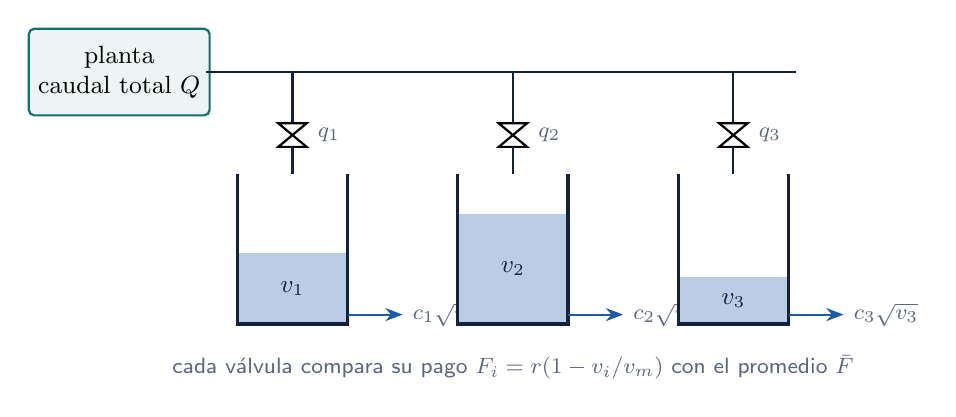
\begin{tikzpicture}[x=1cm,y=1cm]
 \node[bloque=snlteal,minimum width=22mm] (P) at (0,3.2) {planta\\caudal total $Q$};
 \draw[thick,snlnoche] (1.1,3.2) -- (8.6,3.2);
 \foreach \i/\x/\h in {1/2.2/0.9,2/5.0/1.4,3/7.8/0.6}{
   \draw[thick,snlnoche] (\x,3.2) -- (\x,2.55);
   \draw[thick,fill=white] (\x-0.18,2.55) -- (\x+0.18,2.55) -- (\x-0.18,2.25) -- (\x+0.18,2.25) -- cycle;
   \node[nota,right] at (\x+0.2,2.4) {$q_\i$};
   \draw[thick,snlnoche] (\x,2.25) -- (\x,1.9);
   \fill[snlazul!30] (\x-0.7,0) rectangle (\x+0.7,\h);
   \draw[very thick,snlnoche] (\x-0.7,1.9) -- (\x-0.7,0) -- (\x+0.7,0) -- (\x+0.7,1.9);
   \node[etq] at (\x,\h/2) {$v_\i$};
   \draw[->,thick,snlazul] (\x+0.7,0.12) -- ++(0.7,0) node[right,nota]{$c_\i\sqrt{v_\i}$};
 }
 \node[nota] at (5.0,-0.55) {cada válvula compara su pago $F_i=r(1-v_i/v_m)$ con el promedio $\bar F$};
\end{tikzpicture}
\end{document}
